\subsection{Netzwerk scannen}

Um zu überprüfen, welche Dienste laufen, wird ein Portscanner für die Erkennung
benötigt.

\subsubsection{Nmap}

\Nmap{} ist wohl der bekannteste Netzwerkscanner. Er spürt aktive Hosts im Netz auf
und nutzt eine breite Palette an Tests vom normalen TCP/IP-Handshake bis zum
verborgenen TCP-FIN-Scan. Aufgrund der Eigenheiten der TCP/IP-Stacks erkennt
\Nmap{} das Betriebssystem und Dienste.

Unter Free-BSD kann \Nmap{} mit folgender Befehlszeile installiert werden:

\begin{verbatim}
root:~$cd /usr/ports/net/nmap && make install clean
\end{verbatim}

\begin{figure}
\lstinputlisting[language=Metasploit]{listings/nmap.sh}
\caption{Script für dynamischen Portscan: nmap.sh}
\end{figure}

\begin{figure}
\lstinputlisting[language=Metasploit]{listings/nsscan.sh}
\caption{Script zur Namensauflösung: nsscan.sh}
\end{figure}

Mit Hilfe beider des Skriptes nmap.sh (das nsscan.sh intern aufruft) erhält man
eine Liste von Hosts und ihrer offenen Ports im Netzwerk. Die Hosts werden
zunächst als IP Adressen aufgeführt und darunter werden die dazugehörigen DNS
Namen aufgelistet.
\begin{figure}
\lstinputlisting[language=Metasploit]{listings/hostlist}
\caption{Ausgabe von nmap.sh: Die Liste der gefundenen hosts}
\end{figure}

\subsubsection{Zenmap}

Unter \Windows{} gibt es mit \Zenmap{} eine grafische Oberfläche für \Nmap{}. Wenn wir mit dem Befehl 
\lstinline{nmap -sV -T4 -A -v -Pn 172.16.14.0/24} das Netzwerk scannen, dann erhalten wir eine Netzstruktur wie in
 \bildref{netzstruktur}. Wenn wir speziell den Datei- und Webserver betrachten, sehen wir die offenen Ports und Softwareversionen aus \cref{fig:offeneports}.

\bilddateisloppy{netzstruktur}{Netzstruktur}{0.7}

\begin{figure}
 \centering
 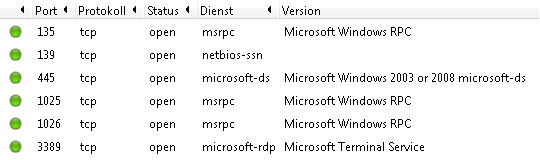
\includegraphics[width=\textwidth,keepaspectratio=true]{Images/dateiserverports}
 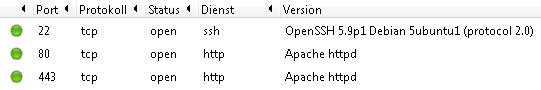
\includegraphics[width=\textwidth,keepaspectratio=true]{Images/webserverports}
 \caption{Offene Ports für Dateiserver (oben) und Webserver (unten)}
 \label{fig:offeneports}
\end{figure}

